\documentclass[a4paper]{article}
\usepackage[normalem]{ulem}
\usepackage{eurosym}
\usepackage[font=small,labelfont=bf]{caption}

%\usepackage{hyperref}

% impostazioni generali
%Tutti gli usepackage vanno qui
\usepackage{geometry}
\usepackage[italian]{babel}
\usepackage[utf8]{inputenc}
\usepackage{tabularx}
\usepackage{longtable}
\usepackage{hyperref}
\usepackage{enumitem}
\usepackage{array} 
\usepackage{booktabs}
\newcolumntype{M}[1]{>{\centering\arraybackslash}m{#1}}
\usepackage[toc]{appendix}
\usepackage{caption}

\hypersetup{
	colorlinks=true,
	linkcolor=blue,
	filecolor=magenta,
	urlcolor=blue,
}
% Numerazione figure
\let\counterwithout\relax
\let\counterwithin\relax
\usepackage{chngcntr}

% distanziare elenco delle figure e delle tabelle
\usepackage{tocbasic}
\DeclareTOCStyleEntry[numwidth=3.5em]{tocline}{figure}% for figure entries
\DeclareTOCStyleEntry[numwidth=3.5em]{tocline}{table}% for table entries


%\counterwithout{table}{section}
%\counterwithout{figure}{section}
\captionsetup[table]{font=small,skip=5pt} 

\usepackage[bottom]{footmisc}
\usepackage{fancyhdr}
\setcounter{secnumdepth}{4}
\usepackage{amsmath, amssymb}
\usepackage{array}
\usepackage{graphicx}

\usepackage{ifthen}

\usepackage{float}
\restylefloat{table}

\usepackage{layouts}
\usepackage{url}
\usepackage{comment}
\usepackage{eurosym}

\usepackage{lastpage}
\usepackage{layouts}
\usepackage{eurosym}

\geometry{a4paper,top=3cm,bottom=4cm,left=2.5cm,right=2.5cm}

%Comandi di impaginazione uguale per tutti i documenti
\pagestyle{fancy}
\lhead{
\includegraphics[scale=0.05]{../../../template/images/logo.png}}
%Titolo del documento
\rhead{\doctitle{}}
%\rfoot{\thepage}
\cfoot{Pagina \thepage\ di \pageref{LastPage}}
\setlength{\headheight}{41pt}
\setcounter{tocdepth}{5}
\setcounter{secnumdepth}{5}
\renewcommand{\footrulewidth}{0.4pt}

% multirow per tabelle
\usepackage{multirow}

% Permette tabelle su più pagine
%\usepackage{longtable}


% colore di sfondo per le celle
\usepackage[table]{xcolor}

%COMANDI TABELLE
\newcommand{\rowcolorhead}{\rowcolor[HTML]{007c95}}
\newcommand{\captionline}{\rowcolor[HTML]{FFFFFF}} %comando per le caption delle tabelle
\newcommand{\cellcolorhead}{\cellcolor[HTML]{007c95}}
\newcommand{\hlinetable}{\arrayrulecolor[HTML]{007c95}\hline}

%intestazione
% check for missing commands
\newcommand{\headertitle}[1]{\textbf{\color{white}#1}} %titolo colonna
\definecolor{pari}{HTML}{b1dae3}
\definecolor{dispari}{HTML}{d7f2f7}

% comandi \textit{Glossario}
\newcommand{\glo}{$_{G}$}
\newcommand{\glosp}{$_{G}$ }


%label custom
\makeatletter
\newcommand{\uclabel}[2]{%
	\protected@write \@auxout {}{\string \newlabel {#1}{{#2}{\thepage}{#2}{#1}{}} }%
	\hypertarget{#1}{#2}
}
\makeatother

%riportare pezzi di codice
\definecolor{codegray}{gray}{0.9}
\newcommand{\code}[1]{\colorbox{codegray}{\texttt{#1}}}


% dati della prima pagina 
% Configurazione della pagina iniziale
\newcommand{\doctitle}{\textit{Glossario}}
\newcommand{\rev}{0.3.1} % versione
\newcommand{\resp}{Ibra Elton} % inserire responsabile
\newcommand{\red}{Corbu Teodor Mihail}
\newcommand{\ver}{Andreetto Alessio}
\newcommand{\uso}{Esterno}
\newcommand{\dest}{\textit{Project Origin}
	\\ Prof. Vardanega Tullio 
	\\ Prof. Cardin Riccardo}
\newcommand{\describedoc}{Glossario contenente i termini per i quali è necessaria una definizione univoca del gruppo \newline \textit{Project Origin} nella realizzazione del progetto \textit{Personal Identity Wallet}}

 % per modificare la prima pagina editare questo file

\makeindex

\makeatletter
\renewcommand\paragraph{
\@startsection {paragraph}{4}{0mm}{-\baselineskip}{.5\baselineskip}{\normalfont \normalsize \bfseries }}
\makeatother

\begin{document}

% Prima pagina
\thispagestyle{empty}
\renewcommand{\arraystretch}{1.3}

\begin{titlepage}
	\begin{center}
		
	
\includegraphics[scale = 0.20]{../../../template/images/logo.png}
	\\[1cm]
	\href{mailto:projectorigin2023@gmail.com}		      	
	{\large{\textit{projectorigin2023@gmail.com} } }\\[2.5cm]
	\Huge \textbf{\doctitle} \\[1cm]
	 \large
			 \begin{tabular}{r|l}
                        \textbf{Versione} & \rev{} \\
                        \textbf{Responsabile} & \resp{} \\
                        \textbf{Redattori} & \red{} \\ 
                        \textbf{Verificatori} &  \ver{} \\
                        \textbf{Uso} & \uso{} \\                        
                        \textbf{Destinatari} & \parbox[t]{5cm}{ \dest{} }
                \end{tabular} 
                \\[3.3cm]
                \large \textbf{Descrizione} \\ \describedoc{} 
     \end{center}
\end{titlepage}

% Diario delle modifiche
\section*{Registro delle modifiche}

\newcommand{\changelogTable}[1]{
	 

\renewcommand{\arraystretch}{1.5}
\rowcolors{2}{pari}{dispari}
\begin{longtable}{ 
		>{\centering}M{0.07\textwidth} 
		>{\centering}M{0.13\textwidth}
		>{\centering}M{0.20\textwidth}
		>{\centering}M{0.17\textwidth} 
		>{\centering\arraybackslash}M{0.30\textwidth} 
		 }
	\rowcolorhead
	\headertitle{Vers.} &
	\centering \headertitle{Data} &	
	\headertitle{Autore} &
	\headertitle{Ruolo} & 
	\headertitle{Descrizione} 
	\endfirsthead	
	\endhead
	
	#1

\end{longtable}
\vspace{-2em}

}

\changelogTable{
0.0.2 & 03-05-23 & Michele Beschin & Analista &  Aggiunti termini al glossario\\
0.0.1 & 02-05-23 & Michele Beschin & Analista &  Creazione struttura documento\\

} % editare questo
\pagebreak

% Indice
{
    \hypersetup{linkcolor=black}
    \tableofcontents
    %\listoffigures %elenco figure
    %\listoftables  %elenco tabelle
}
\pagebreak


% sezioni comuni 
\section{Obiettivi del EUDI Wallet}
L'obiettivo principale del portafoglio europeo di identità digitale proposto è garantire l'accesso a identità digitali affidabili per tutti i cittadini europei, consentendo agli utenti di avere il controllo delle proprie interazioni e della propria presenza online.\\
Può essere visto come una combinazione di diversi prodotti e Trust Services che consente agli utenti di richiedere, ottenere e archiviare in modo sicuro le proprie informazioni consentendo loro di accedere ai servizi online, presentare dati su di loro e firmare o siglare elettronicamente i documenti.\\
Il gruppo eIDAS ha individuato alcune aree di casi d'uso, tra le quali:
\begin{itemize}
    \item Secure and trusted identification to access online services;
    \item Mobility and digital driving licence;
    \item Health;
    \item Educational credentials and professional qualifications;
    \item Digital Finance;
    \item Digital Travel Credential.
\end{itemize}

\section{Definizioni}
\begin{itemize}
    \item \textbf{EUDI}: European Digital Identity;
    \item \textbf{Attribute}: una caratteristica o qualità di una persona fisica o giuridica o di un'entità, in forma elettronica;
    \item \textbf{Issuer}: un Person Identification Data Provider che rilascia PID o un Trust Service Provider che rilascia (Q)EAA.
    \\Nel caso del portafoglio EUDI potrebbero esserci più emittenti per PID e (Q)EAA;
    \item \textbf{PID, Personal Identification Data}: insieme di dati che consentono di stabilire l'identità di una persona fisica o giuridica o di una persona fisica che rappresenta una persona giuridica;
    \item \textbf{(Q)EAA Provider, Qualified Electronic Attestations of Attributes Provider}: un'attestazione elettronica qualificata degli attributi che definiscono una persona, che viene rilasciata da un Qualified Trust Service Provider;
    \item \textbf{QES, Qualified Electronic Signature}: software o hardware configurato utilizzato per creare una firma elettronica;
    \item \textbf{EAAs, Electronic Attestation of Attributes}: un'attestazione in formato elettronico che consente l'autenticazione di attributi.
\end{itemize}







\pagebreak
\section{European Digital Identity Wallet Ecosystem}
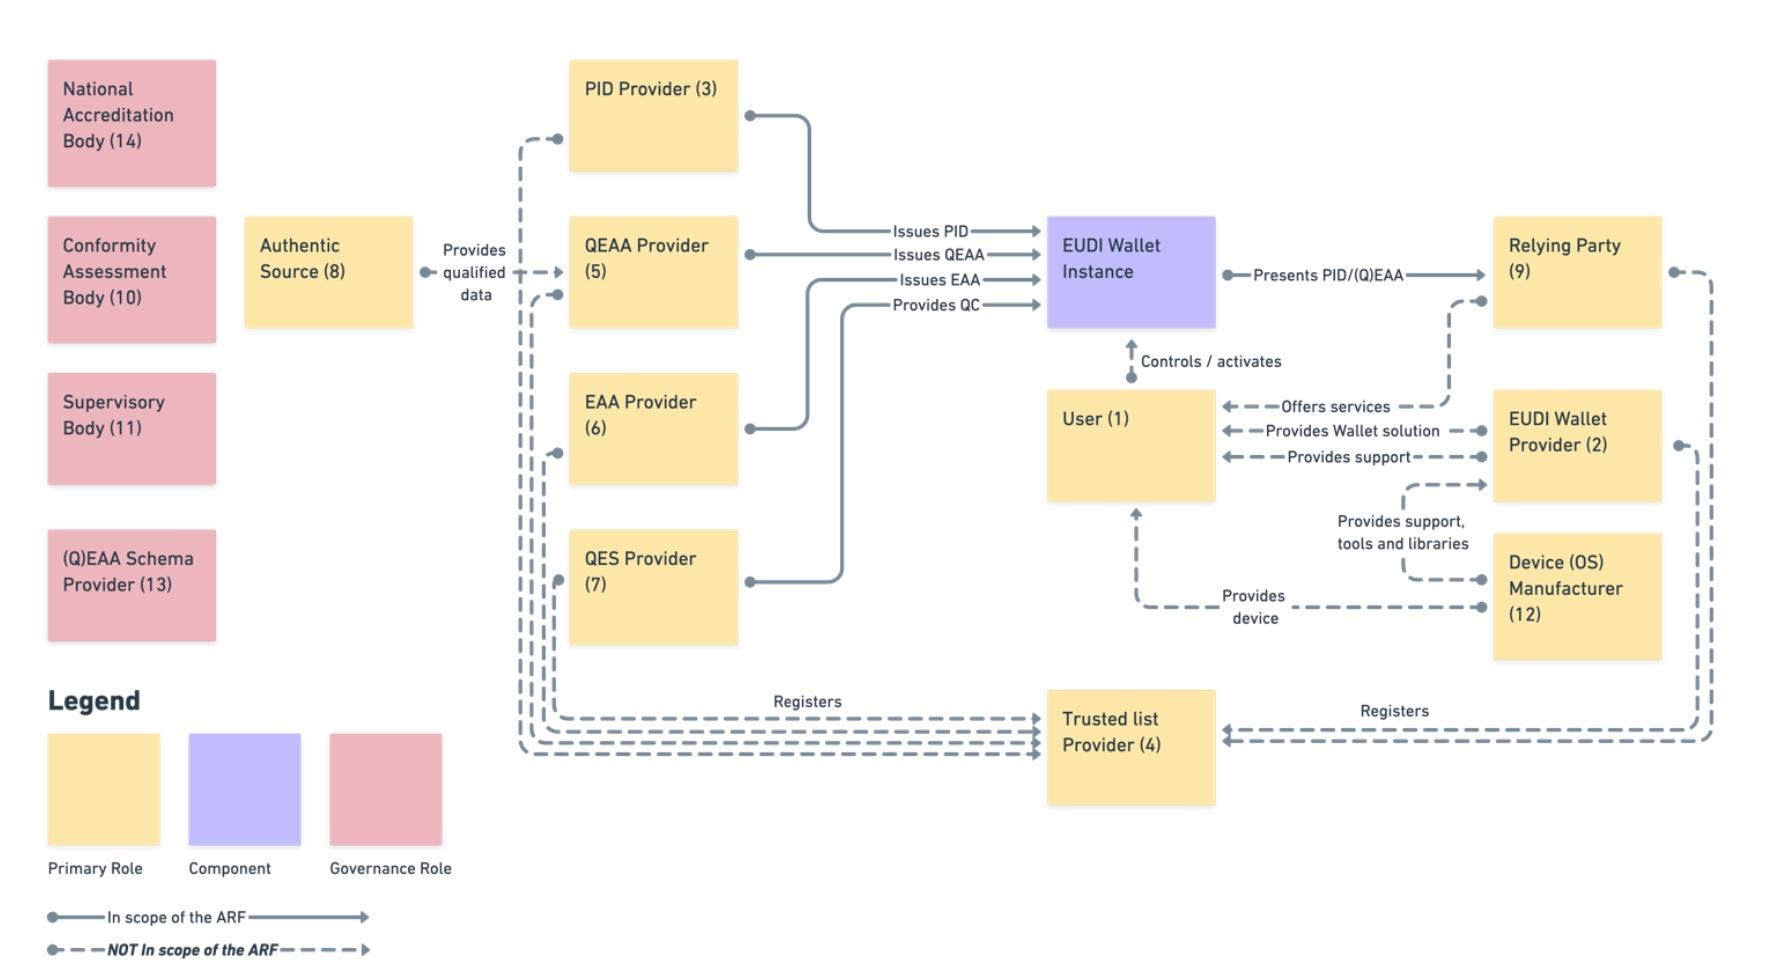
\includegraphics[width=\textwidth]{res/images/EcosistemaEUDI.jpg}
\subsection{Users of EUDI Wallet}
Gli utenti utilizzano il wallet\glo{} EUDI per ricevere, archiviare e presentare attestati (PID, QEAA o EAA) su se stessi, anche per dimostrare la propria identità.
Gli utenti possono creare Qualified Electronic Signatures and Seals (QES) utilizzando un wallet EUDI.
Chi può essere un utente di un wallet EUDI dipende dalla legislazione nazionale.
\subsection{EUDI Wallet Provider}
I fornitori di portafogli EUDI sono Stati membri od organizzazioni incaricate o riconosciute dagli Stati membri che mettono a disposizione il portafoglio EUDI per gli utenti finali.
\subsection{Person Identification Data (PID) Providers}
I fornitori di PID sono entità fidate responsabili di:
\begin{itemize}
    \item Verificare l'identità dell'utente del wallet EUDI;
    \item Rilasciare PID al portafoglio EUDI in un formato comune;
    \item Mettere a disposizione delle Relying Party informazioni per verificare la validità del PID.
\end{itemize}
I fornitori di PID possono ad esempio essere le stesse organizzazioni che oggi rilasciano documenti di identità ufficiali, mezzi di identità elettronica, fornitori di Wallet EUDI ecc.. I fornitori di wallet EUDI possono o meno essere le stesse organizzazioni dei fornitori di PID.
\subsection{Trusted List Providers}
Elenco degli enti attendibili che deve fornire un servizio di registrazione per le entità pertinenti, mantenere un registro e consentire l'accesso di terze parti alle informazioni del registro.
La lista può includere i seguenti fornitori:
\begin{itemize}
    \item Fornitori di Wallet EUDI;
    \item Fornitori di PID;
    \item Fornitori di (QEAA);
    \item Fornitori di (QC);
    \item Fornitori di (EAA).
\end{itemize}
\subsection{Qualified Electronic Attestation of Attributes Providers}
I fornitori QEAA mantengono un'interfaccia per richiedere e fornire QEAA, inclusa un'interfaccia di autenticazione reciproca con i Wallet EUDI e potenzialmente un'interfaccia verso le fonti autentiche per verificare gli attributi.
\subsection{Relying Parties}
Le Relaying Parties sono persone fisiche o giuridiche che fanno affidamento su un'identificazione elettronica o su un Trusted Service.
Nel contesto dei Wallet EUDI, richiedono agli utenti del wallet EUDI gli attributi necessari contenuti nel set di dati PID, QEAA ed EAA per fare affidamento sul portafoglio EUDI, previa accettazione da parte del proprietario del portafoglio (Utente) ed entro i limiti della legislazione e le norme applicabili.
\subsection{PID Attributes per Persone Fisiche}
\begin{longtable}{|c|c|c|}
    \hline
    \textbf{Mandatory eIDAS Attributes} & \textbf{Optional eIDAS Attributes} & \textbf{Optional attributes} \\
    \hline
    \endfirsthead
    
    \multicolumn{3}{c}%
    {\tablename\ \thetable\ --\ Continuazione dalla pagina precedente} \\
    \hline
    \textbf{Mandatory eIDAS Attributes} & \textbf{Optional eIDAS Attributes} & \textbf{Optional attributes} \\
    \hline
    \endhead
    
    \hline \multicolumn{3}{r}{{Continua nella pagina successiva}} \\
    \endfoot
    
    \hline
    \endlastfoot
    
    Current Family Name	 & Family Name at Birth & Nationality/Citizenship \\
    Current First Names & First Names at Birth &  \\
    Date of Birth & Place of Birth & Optional attributes used at national level \\
    Unique Identifier & Current Address & \\
     & Gender & \\    
    \end{longtable}
    L'attestazione PID deve contenere le seguenti informazioni:
    \begin{itemize}
        \item informazioni necessarie per identificare il PID Provider;
        \item informazioni necessarie per eseguire un controllo di integrità e autenticità dei dati;
        \item informazioni necessarie per eseguire i controlli dello stato di validità dell'attestato;
        \item Deve rispettare il ISO/IEC 18013-5:2021 e il W3C Verifiable Credentials Data Model 1.1. e codificato in JSON.
    \end{itemize}
    Stesse informazioni devono essere garantite per i (Q)EAA.
    Tipi di funzionamento del EUDI Wallet:
    \begin{itemize}
        \item Locale. Può funzionare in maniera supervisionata o non supervisionata tramite un contatto fisico (QRCode, NFC) e questo funzionamento può accadere anche senza connessione a internet.\\
        Per protocollo di comunicazione si dovranno seguire quelli dettagliati nel
        ISO/IEC 18013-5:2021;
        \item Remote. Può funzionare over the internet, con sistemi in cui il wallet è utilizzato per garantire sessioni di autenticazione e dove i certificati possono essere utilizzati e consumati dallo stesso sito che li richiede.
        \\Per questo funzionamento come protocollo di comunicazione si dovrà utilizzare OpenID4VP, in particolare questo è un Attestation exchange protocol.
        \\Per l'Issuer che forniscono certificati al Wallet si dovranno utilizzare il protocollo OpenID4VCI.
    \end{itemize}

    Possono essere scenari di utilizzo:
    \begin{itemize}
        \item User e Relying Party sono entrambi online;
        \item Solo User è online;
        \item Solo Relying Party è online;
        \item User e Relying Party sono entrambi offline.
    \end{itemize}
\section{Fonti}
\href{https://digital-strategy.ec.europa.eu/en/library/european-digital-identity-wallet-architecture-and-reference-framework}{https://digital-strategy.ec.europa.eu/en/library/european-digital-identity-wallet-architecture-and-reference-framework}\\
\href{https://github.com/eu-digital-identity-wallet/architecture-and-reference-framework}{https://github.com/eu-digital-identity-wallet/architecture-and-reference-framework}


\end{document}



